\section{Introduction}
Recommendation systems are a vital component of the modern Web.  They
help readers effectively navigate otherwise unwieldy archives of
information and help websites direct users to items---movies,
articles, songs, products---that they will like.  A recommendation
system is built from historical data about which items each user has
consumed, be it clicked, viewed, rated, or purchased. First, it
uncovers the behavioral patterns that characterize various types of
users and the kinds of items they tend to like.  Then, it exploits
these discovered patterns to recommend future items to its users.

In this paper, we develop Hierarchical Poisson factorization (HPF) for
generating high-quality recommendations. Our algorithms easily scale
to massive data and significantly outperform the existing methods. We
show HPF is tailored to real-world properties of user behavior data:
the heterogeneous interests of users, the varied types of items, and a
realistic distribution of the finite resources that users have to
consume these items.

%% \begin{figure*}[th]
%% \centering
%% \vspace{0.1cm}
%% \small
%% \begin{tabular}{c}
%% \bf{``Action''}\\
%% \midrule
%% The Matrix\\
%% The Matrix: Reloaded\\
%% Spider-Man\\
%% X2: X-Men United\\
%% \bottomrule
%% \end{tabular}
%% \begin{tabular}{c}
%% \bf{``Indie Comedy, Romance''}\\
%% \midrule
%% Grosse Pointe Blank\\
%% Four Weddings and a Funeral\\
%% High Fidelity\\
%% Much Ado About Nothing\\
%% \bottomrule
%% \end{tabular}
%% \begin{tabular}{c}
%% \bf{``80's Science Fiction''}\\
%% \midrule
%% Star Wars: Episode IV: A New Hope\\
%% Star Wars: Episode VI: Return of the Jedi\\
%% Star Wars: Episode V: The Empire Strikes Back\\
%% Back to the Future Part II\\
%% \bottomrule
%% \end{tabular}

%% \vspace{0.5cm}

%% \centering
%% 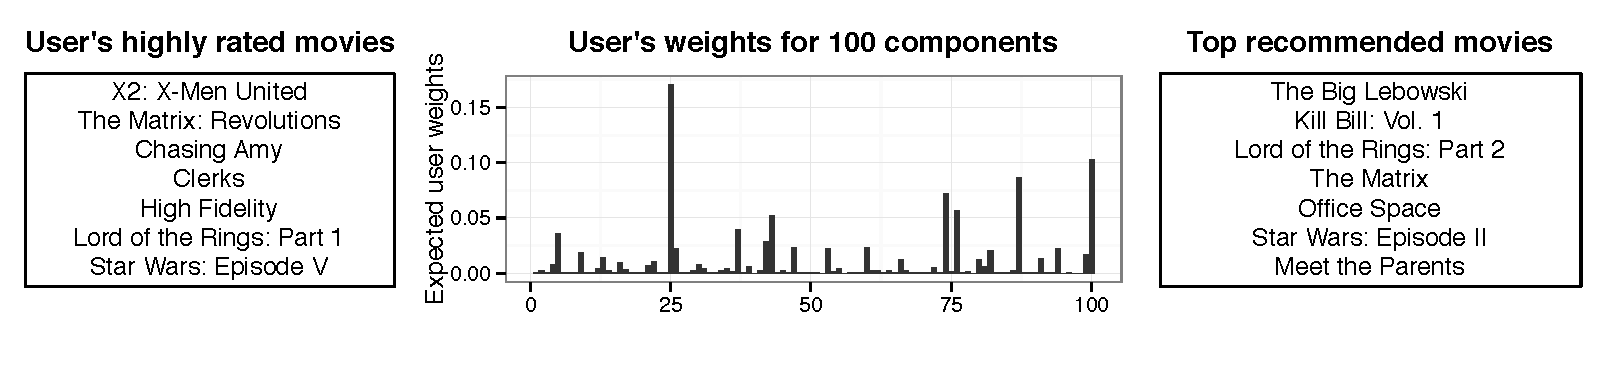
\includegraphics[width=0.8\textwidth]{figures/netflix-exploratory.pdf}
%% \caption{The top panel shows the top movies in 3 components for a
%%   user from the Netflix data set. The bottom panel is an illustration
%%   showing a subset of the highly rated movies by this user, and the
%%   right panel shows movies recommended to the user by our
%%   algorithm. The expected user's $K$-vector of weights $\theta_u$,
%%   inferred by our algorithm is shown in the middle panel.}
%% \label{fig:netflix-illustration}
%% \end{figure*}

%% \myfig{netflix-illustration} illustrates Poisson factorization on data
%% from Netflix.  The Netflix data contains the ratings of 480,000 users
%% on 17,000 movies, organized in a sparse matrix of 8.16B cells (and
%% containing 250M ratings).  From these data, we extract the patterns of
%% users' interests and the movies that are associated with those
%% interests.  The left panel illustrates some of those patterns---the
%% algorithm has uncovered action movies, independent comedies, and 1980s
%% science fiction.  The top panel illustrates how we can use these
%% patterns to form recommendations for an (imaginary) user.  This user
%% enjoys various types of movies, including fantasy (``Lord of the
%% Rings''), classic science fiction (``Star Wars: Episode V''), and
%% independent comedies (``Clerks'', ``High Fidelity'').  Of course, she
%% has only seen a handful of the available movies.  PF first uses the
%% movies she has seen to infer what kinds of movies she is interested
%% in, and then uses these inferred interests to suggest new movies.  The
%% list of movies at the bottom of the figure was suggested by our
%% algorithm. It includes other comedies (such as ``The Big Lebowski'')
%% and other science fiction (such as ``Star Wars: Episode II'').

In more detail, HPF is a probabilistic model of users and items.  It
associates each user with a latent vector of preferences, each item
with a latent vector of attributes, and constrains both sets of
vectors to be sparse and non-negative. The model assumes that each
cell of the observed behavior matrix is drawn from a Poisson
distribution---an exponential family distribution over non-negative
integers---whose parameter is a linear combination of the
corresponding user preferences and item attributes.  The main
computational problem is posterior inference: given an observed matrix
of user behavior, we would like to discover the latent attributes that
describe the items and the latent preferences of the users, which we
can then use to make predictions and recommendations.

%% recys-prem !!! removed paragraph below (references fig 1)

%%  For example, the
%% components in \myfig{netflix-illustration} (left) illustrate the top
%% items for specific attribute dimensions and the plot in
%% \myfig{netflix-illustration} (middle) illustrates the estimated
%% preference vector for the given user.  A spike in the preference
%% vector implies that the user tends to like items with the
%% corresponding latent attribute.

This inferential computation is common to many variants of matrix
factorization.  We found, however, that HPF enjoys significant
quantitative advantages over classical methods over a variety of
\emph{implicit feedback} data sets. \myfig{precision_recall} shows
that HPF performs significantly better than competing
methods---including the industry standard of matrix factorization with
user and item biases (MF)---for large data sets of Netflix users
watching movies, Last.FM users listening to music, scientists reading
papers, and \textit{New York Times} readers clicking on articles.

{\bf Comparison to Gaussian MF.} Many of the leading MF methods are
based on Gaussian likelihoods (i.e., squared loss). When applied to
explicit data, Gaussian models are fit only to the observed
ratings~\cite{Koren:2009} and infer distributions over user
preference. For each user, the items she did not consume, i.e., the
zero observations, are treated as ``missing data''. Gaussian models
make up the state of the art in this setting~\cite{Salakhutdinov:2008,
  Salakhutdinov:2008a,Koren:2009}.

In implicit data sets of user consumption, there is a fundamental
asymmetry that allows one to infer which items a user consumed, and
therefore liked, but not which items a user did not
like~\cite{Hu:2008p9402}. In this setting, Gaussian MF applied to all
observations gives equal weight to consumed and unconsumed items.
Consequently, when faced with a sparse matrix and implicit feedback,
matrix factorization places more total emphasis on the unconsumed
user/item pairs.

To address this limitation of Gaussian MF, researchers have patched it
in complex ways. There are two main approaches. The first approach,
proposed by \cite{Hu:2008p9402}, is to treat the unconsumed items with
greater uncertainty and increase confidence as the rating for an item
increases. This converts the raw observations into two separate
quantities with distinct interpretations: user preferences and
confidence levels. Hu et al.~\cite{Hu:2008p9402} present an
alternating least squares algorithm that considers all observations
but whose per-iteration complexity is still linear in the number of
non-zero observations. A main disadvantage of this method is that the
assignment of per-observation confidence weights requires exhaustive
search via cross-validation, or other model selection methods, which
is impractical on massive data sets.
%% For scalability, the method assigns a single confidence level
%% parameter for all zero observations. This simpler treatment fails
%% to capture that the vast majority of observations are zero not
%% because the user disliked them, but because they have not even
%% considered them.

The second approach is to randomly synthesize negative
examples~\cite{Dror:2012a, Gantner:2012p9364, Paquet:2013p9197}. In
this approach, unconsumed items are subsampled for each user to
balance out the consumed items. As Dror et al.~\cite{Dror:2012a} note,
it is unclear how to balance these two sets of items. Do we use an
equal number of consumed and consumed items, or do we use the full set
of unconsumed items~\cite{Cremonesi:2010, Hu:2008p9402}?  Further, the
subsampling of negative or unconsumed items is often expensive, and
can account for a substantial fraction of resources devoted to model
fitting.

One problem with most Gaussian models is they do not capture that
users have limited resources to consume, view, or rate items from a
vast number of options. 
%% They either interpret all unconsumed observations as having high
%% uncertainty around them---conflating zeros due to limited user
%% resources and zeros due to disliking an item---or they subsample
%% unconsumed items to learn a balanced user profile. Neither approach
%% treats the zero observations as a signal for the limited rate at which
%% each user consumes items.
In contrast, Poisson factorization (PF) captures real consumption
data, specifically that users have finite (and varied) resources with
which to consume items.  To see this, we can rewrite the model as a
two stage process where a user first decides on a budget of how many
movies to watch and then spends this budget on movies of interest. If
the model accurately captures the distribution of budgets then
consumed items carry more weight than unconsumed items, because
unconsumed items can be partially explained by a lack of resources. We
conjecture that matrix factorization methods based on the Gaussian
model systematically overestimate the users' budgets, and we confirm
this hypothesis in \mysec{eval} using a posterior predictive
check~\cite{Gelman:1996}. This misfit leads to an overweighting of the
zeros, which explains why practitioners require complex methods for
downweighting
them~\cite{Hu:2008p9402,Gantner:2012p9364,Dror:2012a,Paquet:2013p9197}.
Poisson factorization does not need to be modified in this way.

Further, the HPF algorithm retains the linear-scaling of Gaussian MF
with downweighted zeros~\cite{Hu:2008p9402}. HPF algorithms only need
to iterate over the consumed items in the observed matrix of user
behavior. This follows from the mathematical form of the Poisson
distribution.  In contrast, the subsampling-based Gaussian MF
methods~\cite{Gantner:2012p9364, Dror:2012a,Paquet:2013p9197} must
iterate over both positive and negative examples in the implicit
setting. This makes it difficult to take advantage of data sparsity to
scale to massive data sets.

Finally, unlike Gaussian MF which typically provides dense latent
representations of users and items, PF models provide sparse latent
representations. This property arises from the PF log-likelihood which
can be shown to minimize the information (Kullback-Leibler) divergence
under NMF~\cite{Cemgil:2009}, and from the Gamma priors on user
preferences and item attributes that we place in the HPF model of
\mysec{model}.

{\bf Recent extensions.}
Building on the HPF model and algorithm we present in this paper,
recent work has proposed a joint model of article text and reader
preferences~\cite{gopalan2014content}. This model takes advantage of
the sparse, non-negative representations in PF, which are useful in
capturing different types of discrete data, such as word counts and
user ratings. Further, they exploit the additive properties of
independent Poisson random variables to capture dependencies between
discrete data, for example, the dependence of user ratings of an
article on its content. Another recent work proposes a Bayesian
nonparametric model~\cite{gopalan2014bayesian} that adapts the
dimensionality of the latent representations, learning the preference
patterns (and their number) that best describe the users. Both models
exploit the scalability of PF algorithms to study massive data sets.
These extensions testify to the modeling flexibility of PF models.

We review other related work below before discussing details of the
Poisson factorization model, including its statistical properties and
methods for scalable inference.

%%
%%\begin{figure}
%%\centering
%%\includegraphics[width=0.8\columnwidth]{figures/movielens-user.pdf}\\
%%\includegraphics[width=0.8\columnwidth]{figures/movielens-item.pdf}\\
%%\caption{The weights of the randomly chosen user $U$ (Top) in the
 %% movielens data set and the weights of her top recommended movie
  %%\emph{Shakespeare in Love} (Bottom) are shown. User $U$ views a
  %%variety of movies, and her weights span a range of factor. User $U$
  %%had 184 views in the data set of movies ranging from Drama, Comedy,
  %%Thriller to Musical. Of these movies, 126 were either 4 or 5
  %%stars. Movies are generally characterized by a sparse set of
  %%factors.}
%%\end{figure}



%% \begin{figure*}[t!]
%% 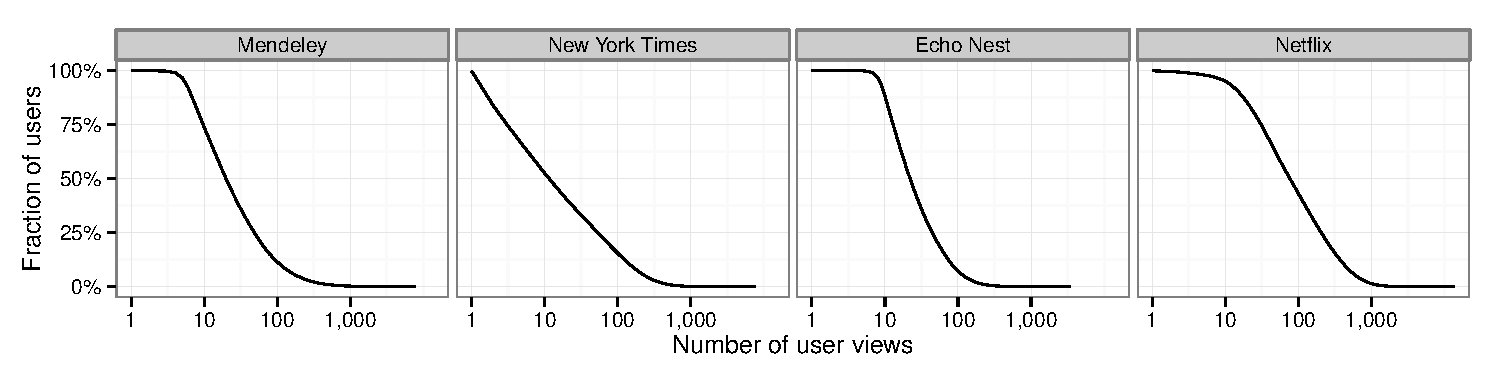
\includegraphics[width=\textwidth]{figures/user_activity_cdf.pdf}
%% \caption{Empirical complimentary cumulative distributions of user
%%   activity on each data set. Each curve shows the fraction of users
%%   who have consumed at least a given number of items. For instance,
%%   slightly less than half of all Netflix users have rated at least
%%   100 movies.}
%% \label{fig:marginals}
%% \end{figure*}


%% \begin{figure*}[t!]
%%   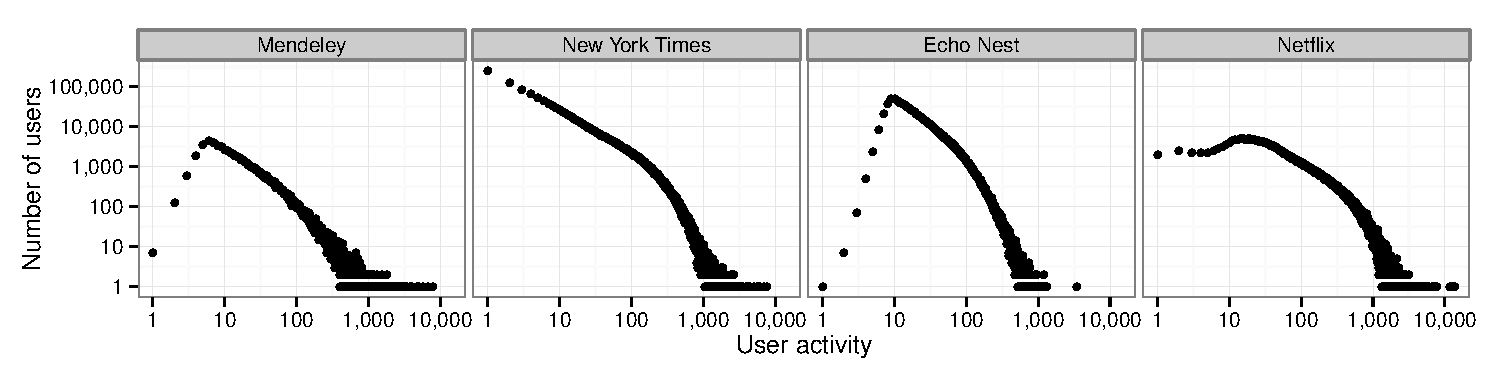
\includegraphics[width=\textwidth]{figures/user_activity.pdf}
%%   \caption{Empirical distributions of user activity on each
%%     dataset. Each plot shows the number of users who have rated a given
%%     number of items. For instance, slightly less than half of all
%%     Netflix users have rated at least 100 movies.}
%% \label{fig:marginals}
%% \end{figure*}

%% \begin{figure*}[t!]
%% 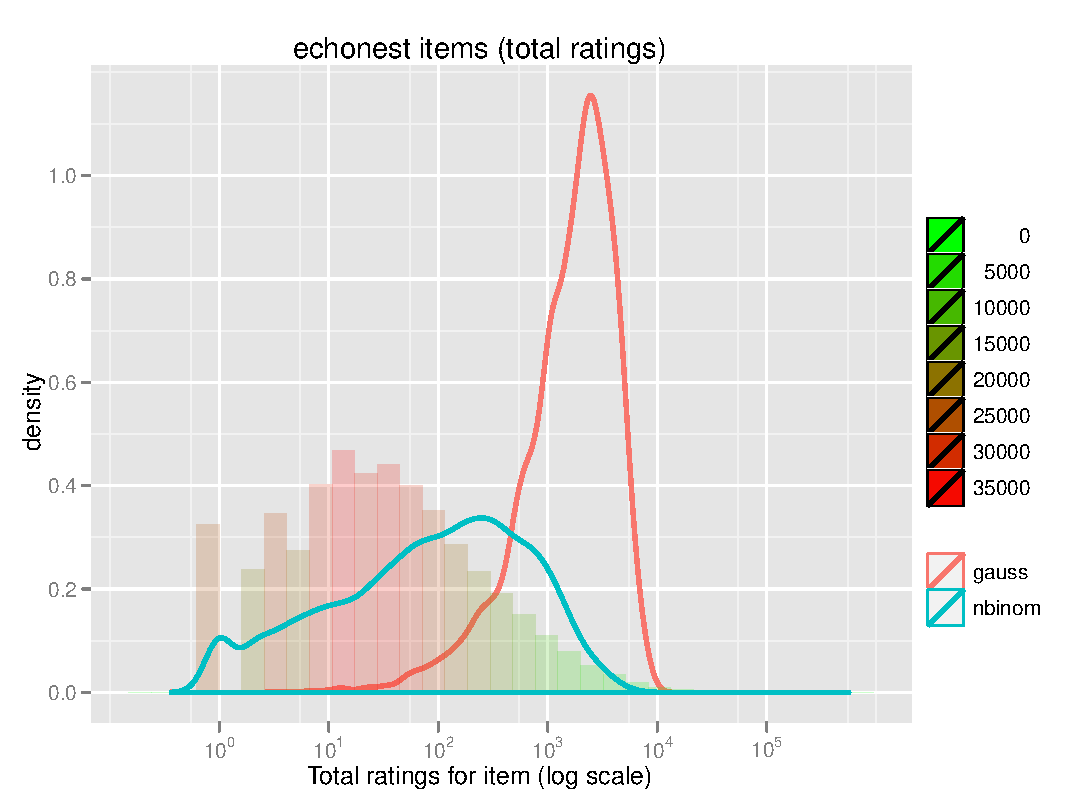
\includegraphics[width=0.33\textwidth]{figures/marginals/echonest.pdf}
%% 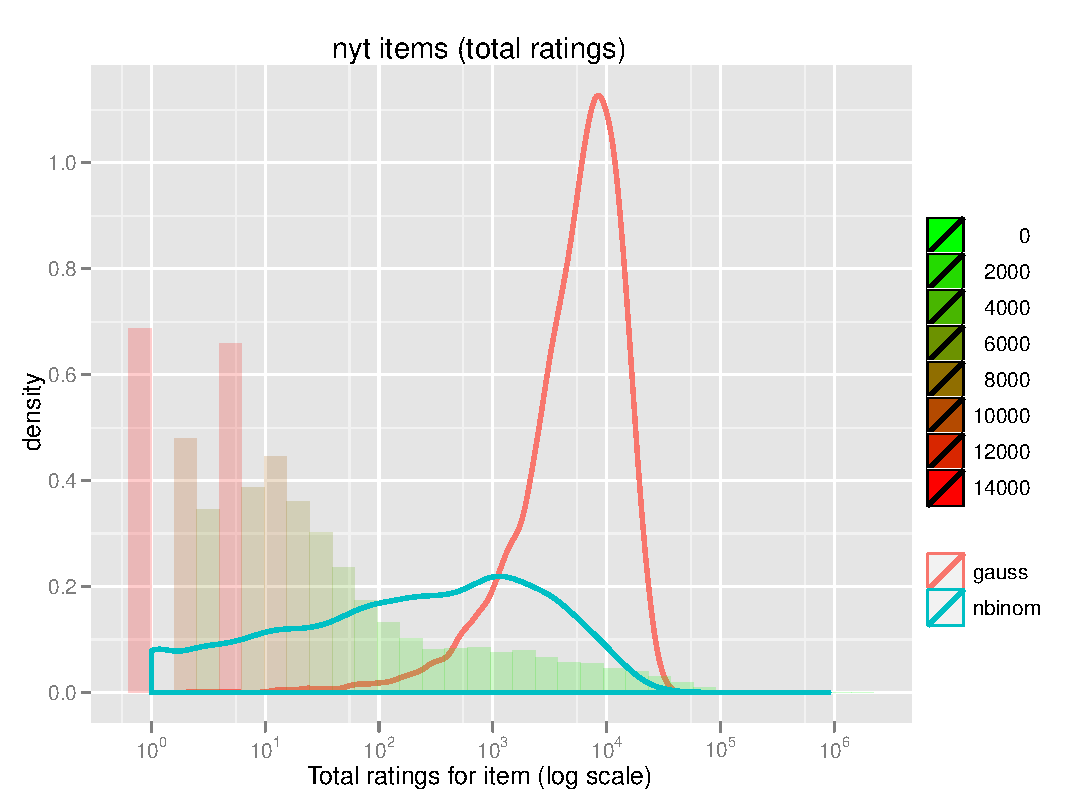
\includegraphics[width=0.33\textwidth]{figures/marginals/nyt.pdf}
%% 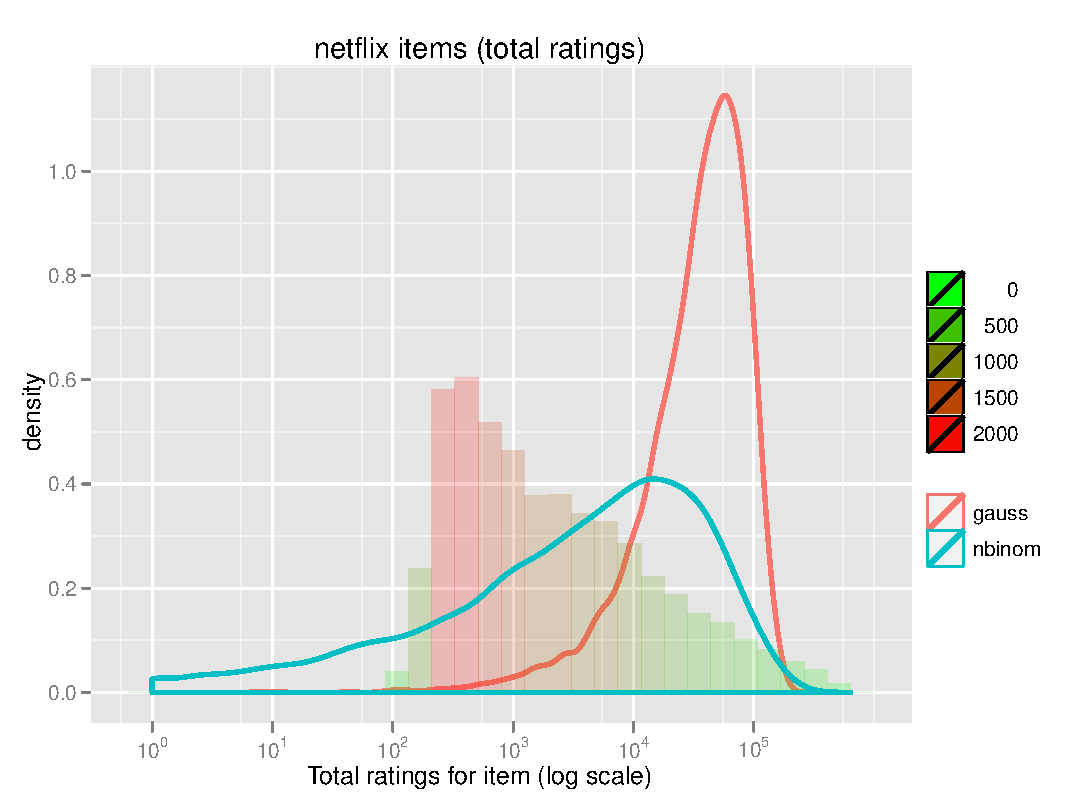
\includegraphics[width=0.33\textwidth]{figures/marginals/netflix.pdf}
%% \caption{Empirical distribution of item popularity on real datasets,
%%   with fitted negative binomial and Gaussian distributions. The
%%   distributions were fit using maximum likelihood estimation. The
%%   negative binomial places significant probability mass on the left
%%   tail, i.e., items with few ratings. The colored bars show that such
%%   items are the most frequent. In contrast, the Gaussian distribution
%%   places negligible mass on the left tail and mainly captures popular
%%   items. The mode of the negative binomial distribution is also closer
%%   to the empirical mode than the Gaussian distribution.}
%% \label{fig:marginals}
%% \end{figure*}

%% Further speed-ups using stochastic variational
%% inference~\cite{Hoffman:2013} let us fit Poisson factorization models
%% to massive data.

